\RequirePackage[T1]{fontenc}
\documentclass[conference,10pt,letterpaper]{IEEEtran}

\renewcommand{\ttdefault}{lmtt}
\usepackage{amsmath,amssymb,graphicx,booktabs,cite}
\usepackage{tikz}
\usepackage[ruled,vlined,linesnumbered]{algorithm2e}
\SetKwInOut{Input}{Input}
\SetKwInOut{Output}{Output}
\SetKwProg{Stage}{}{}{}
\DontPrintSemicolon
\SetAlgoNlRelativeSize{-1}
\SetInd{0.4em}{0.75em}
\usetikzlibrary{arrows.meta,positioning}
\usepackage{pgfplots}
\usepgfplotslibrary{groupplots}
\pgfplotsset{compat=1.18}
\usepackage[hidelinks]{hyperref}
\hypersetup{pdfauthor={},pdftitle={Exposing Inter-Sample and Intra-Search Parallelism in Layer-Aware Lookahead Construction for 3D FPGA Routing}}
\makeatletter
\newcommand{\tableinput}[1]{\@@input #1 }
\makeatother
\newtheorem{proposition}{\bfseries Proposition}
\title{Exposing Inter-Sample and Intra-Search Parallelism in Layer-Aware Lookahead Construction for 3D FPGA Routing}
\author{\IEEEauthorblockN{Anonymous Authors\\{\small Internal review --- partial measured cohort}}}
\begin{document}\maketitle
\begin{abstract}A change to a 3D FPGA routing-resource graph or its indexed costs can require a fresh lookahead table before routing. Each sampled search contributes a source-relative delay and congestion pair to this table. We identify two opportunities for parallel execution. STRICT issues private native searches across group boundaries and consumes their results in their original order. Under explicit conditions on recording, ties and interpolation, it reproduces the native wire table. ALT changes the search rule to process complete FP32 labels in bucket waves, with CPU and CUDA implementations of the same rule. A profile on 40 BNN samples shows how wider waves trade additional edge work for fewer synchronization rounds. We specify a single-worker native evaluation on three complete two-layer graphs and distinguish construction from complete fixed-input routing time. Unified runtime and route-quality measurements are pending.
\end{abstract}
\begin{IEEEkeywords}3D FPGA, routing lookahead, parallel algorithms, CPU/GPU, source-relative costs\end{IEEEkeywords}
\section{Introduction}
Architecture exploration changes segment lengths, switch patterns and the resources available for crossing dies. A router evaluating a candidate architecture needs estimates for reaching pins on each destination layer~\cite{lazagna,flatland,multidie}. A table built for a previous graph can be reused only when its construction inputs remain compatible. Otherwise the evaluator pays for another set of sample searches before negotiated routing begins.

These searches carry two kinds of ordering. A sample has a particular source and records costs relative to that source. Its contribution must reach the right cell, and equal delays require an ordered choice of congestion representative. Yet an independent sample can begin before all searches in the preceding group finish. A second opportunity arises inside a search. Many edges can propose updates simultaneously if the implementation defines when those proposals become visible and which representative survives.

We derive a bounded native sample schedule (STRICT) and a separately qualified bucket-wave search rule (ALT). STRICT exposes cross-sample parallelism on CPUs. ALT exposes enough work within a sample to support both CPU and GPU implementations. Their integration into native VPR allows us to distinguish search service, complete construction and the full fixed-input routing process. The comparison tracks changes in wire-map representatives alongside route legality and timing quality.

\section{Problem and Parallelism Boundary}
\subsection{Layer-Aware Construction}
Let $G=(V,E)$ be the directed routing-resource graph (RRG), with $N=|V|$ nodes and $M=|E|$ edges. Nodes carry resource type, layer, geometry and an indexed delay/congestion cost $w(v)=(d_v,q_v)$. The graph contains planar and cross-layer channels as well as logic, memory and DSP connectivity~\cite{third_dimension,multidie}. PathFinder-style negotiation resolves contention~\cite{pathfinder}; VPR consumes lookahead costs during routing~\cite{vtr8,vtr9}. We accelerate construction of the sampled wire table~\cite{diversity}, not negotiated routing itself.

A key $g=(\ell_s,\sigma,\tau)$ identifies each group in $\mathcal G$ by source layer, segment type and channel type. Native enumeration yields $J$ jobs indexed by $a$, each retaining group $g(a)$, ordinal, source RR node $s_a=s_{g,j}$ and recording context. One search covers all target layers. Its map $\phi_a(v)$ assigns an eligible IPIN to a source-relative cell $u=(\ell_t,\Delta x,\Delta y)$ or returns $\bot$ when geometry excludes it. A grid of width $X$, height $Y$ and $L$ layers has $C=LXY$ result cells per sample.

An eligible recorded pin contributes one path's accumulated delay $d$ and indexed resource base cost $q$. A cell $R_a[u]$ remains missing if no eligible visit records it before search termination. Native insertion $\oplus$ fills a missing cell or replaces its pair on strictly smaller delay. For each group,
\begin{equation}
 A_g[u]=\mathop{\bigoplus}_{a:g(a)=g}^{\text{native order}}R_a[u],\qquad
 F=\mathcal I\bigl(\mathcal C(\{A_g\})\bigr).
\end{equation}
$\mathcal C$ and $\mathcal I$ denote native group writes and interpolation in their prescribed interleaving and missing-cell scan order. The table is indexed by $(\ell_s,\ell_t,\tau,\sigma,\Delta x,\Delta y)$. Source/OPIN preprocessing and derived minima remain in the outer computation.

\subsection{Necessary Dependencies and Removable Barriers}
\begin{figure}[t]
\centering
{\footnotesize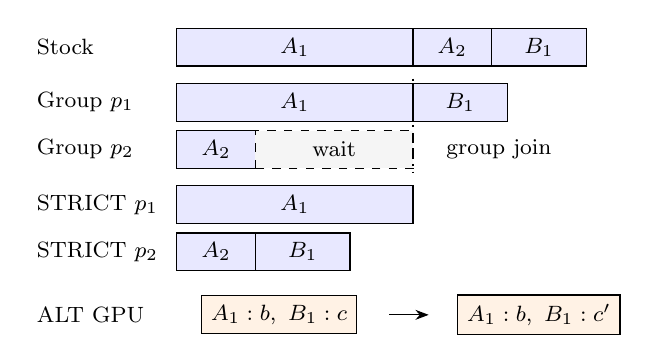
\begin{tikzpicture}[x=1mm,y=1mm,font=\footnotesize,
  bar/.style={draw,fill=blue!9},wait/.style={draw,dashed,fill=gray!8}]
\foreach \yy/\txt in {0/Stock, -7/Group $p_1$, -13/Group $p_2$, -20/STRICT $p_1$, -26/STRICT $p_2$}
 \node[anchor=west] at (0,\yy) {\txt};
\foreach \start/\stop/\yy/\job in {19/49/0/$A_1$,49/59/0/$A_2$,59/71/0/$B_1$,19/49/-7/$A_1$,49/61/-7/$B_1$,19/29/-13/$A_2$,19/49/-20/$A_1$,19/29/-26/$A_2$,29/41/-26/$B_1$}{
 \draw[bar] (\start,\yy-2.4) rectangle (\stop,\yy+2.4);
 \node at ({(\start+\stop)/2},\yy) {\job};}
\draw[wait] (29,-15.4) rectangle (49,-10.6);
\node at (39,-13) {wait};
\draw[dotted,thick] (49,-4)--(49,-16);
\node[anchor=west] at (52,-13) {group join};
\node[anchor=west] at (0,-34) {ALT GPU};
% Illustrative sample-local keys in two successive GPU batch rounds.
\node[draw,fill=orange!10] at (32,-34) {$A_1:b,\ B_1:c$};
\node[draw,fill=orange!10] at (65,-34) {$A_1:b,\ B_1:c'$};
\draw[->,>=Stealth] (46,-34)--(51,-34);
\end{tikzpicture}
}
\caption{Illustrative schedules for three samples. With Group, a worker waits for $A_1$ before starting $B_1$. With STRICT, $A_2$ and $B_1$ finish before $A_1$; their results wait for native-order consumption. In successive ALT GPU rounds $A_1$ can reopen bucket $b$ while $B_1$ advances from $c$ to $c\prime$.}\label{fig:contracts}
\end{figure}
For point-like locations on one row, starts at $x=0$ and $5$ reaching a pin at $x=6$ record displacements 6 and 1. A multi-source search retaining only the cheaper path loses one contribution. Within a cell, equal delays preserve the earlier sample's entire pair. For native-order contributions $(5,9),(5,3),(6,1)$, the winner is $(5,9)$. Consuming the second first gives $(5,3)$, and separate field minima give $(5,1)$, a pair absent from all three paths.

In the locked Stock path, \texttt{get\_routing\_cost\_map} iterates over sampled nodes and calls a Dijkstra flood for each~\cite{lockedvtr}. Each search can instead read shared costs and maintain private labels. It can start before the preceding group joins (Fig.~\ref{fig:contracts}). Changing priority extraction inside a sample can alter its representative and requires a separate search rule.

\subsection{Lookahead Construction in FPGA Routers}
Sharma and Hauck~\cite{adaptive_astar} reduce table storage by clustering wires and searching from each cluster as a single source. Petelin and Betz~\cite{diversity} sample individual wires by type and orientation. For each displacement they record the smallest observed delay and its associated path cost. AIR uses map-based estimates to guide adaptive incremental routing~\cite{air}. The associated path cost in our baseline follows the sampled-wire representation of Petelin and Betz. For 2.5D interposer fabrics, Poolad et al.~\cite{multidie} separate the intra-die estimate from the cost of crossing each intervening die boundary.

These choices determine which costs a router can look up. Building a layer-aware map also requires scheduling the sampled searches. Singer et al.~\cite{multiqueue} evaluate parallel connection searches and suggest using parallel Dijkstra searches to sample more starting wires. We hold the sampled starts fixed. STRICT overlaps native searches while preserving their ordered contributions. ALT processes updates within each search in parallel and checks how the resulting cost pairs affect routed circuits.

\section{Two Parallelization Regimes for Lookahead Construction}
\begin{figure}[t]
\centering
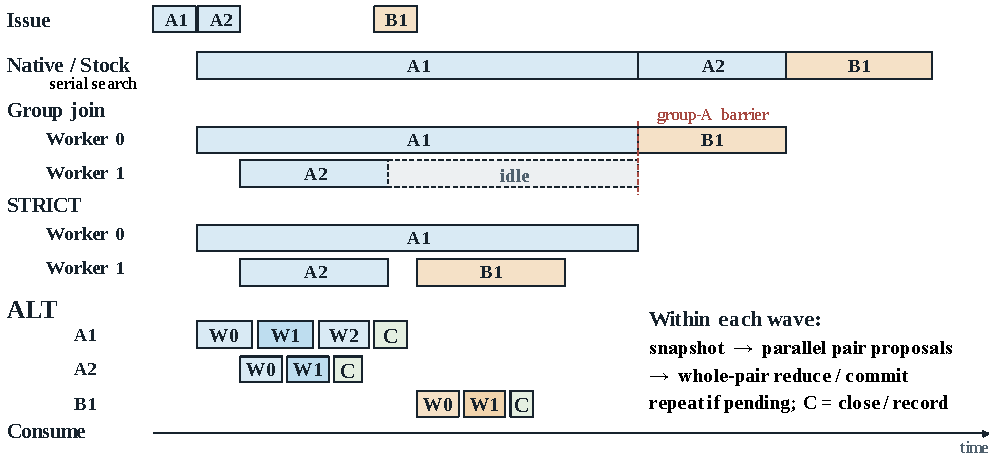
\includegraphics[width=\columnwidth]{figures/timeline.pdf}
\caption{Illustrative schedules for samples $A_1,A_2,B_1$. Group waits at the group boundary. STRICT can issue $B_1$ while $A_1$ is active and still consume in native order. Within an ALT sample, $W_i$ denotes a wave and C marks bucket closure.}\label{fig:contracts}
\end{figure}
\begin{figure*}[t]
\centering
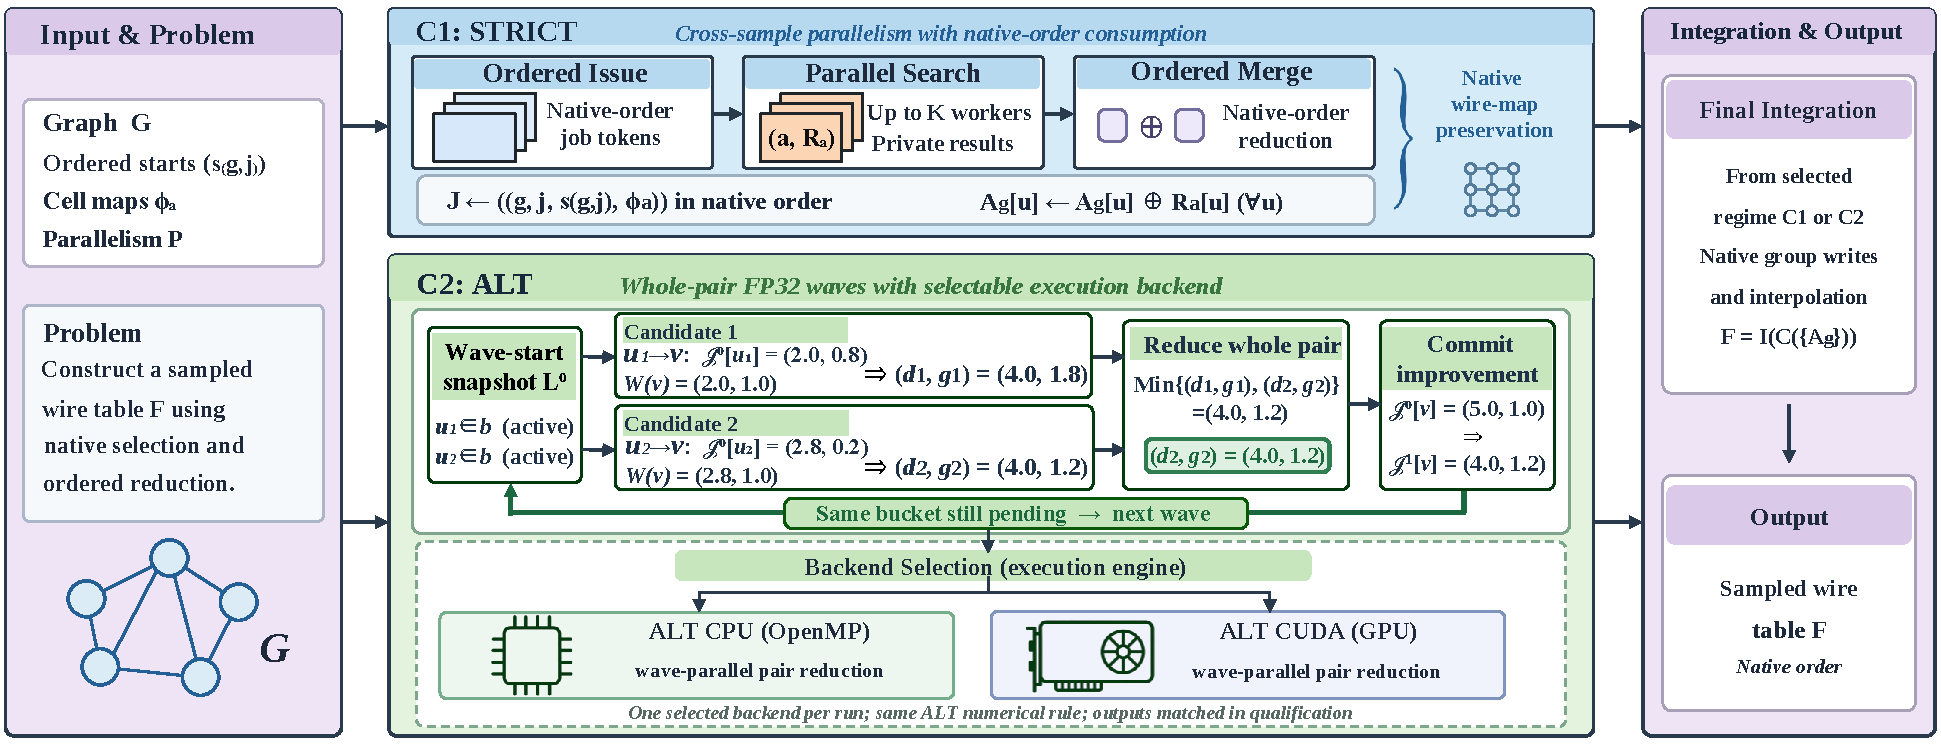
\includegraphics[width=\textwidth]{figures/framework.pdf}
\caption{Layer-aware lookahead construction. In C1, $P$ counts workers and $K$ bounds live tokens. Proposition~\ref{prop:strict} gives the native-map guarantee. C2 distributes samples across CPU workers or processes active nodes in parallel on the GPU (CUDA), using the same whole-pair rule. The selected regime returns sample results for native group writes and interpolation.}\label{fig:framework}
\end{figure*}

Figure~\ref{fig:contracts} compares schedules. Figure~\ref{fig:framework} follows a batch from its ordered starts to the native wire table.
\subsection{C1: Private Samples and Ordered Consumption}
In Algorithm~\ref{alg:c1}, token $a$ identifies the group, ordinal, source and cell map across group boundaries. Worker $p$ resets its private queue, visited costs and expanded bits in $S_p$. Its flood reads the shared graph with native geometry, edge eligibility and arithmetic.

\begin{algorithm}[t]\footnotesize
\caption{Bounded STRICT sample pipeline (C1)}\label{alg:c1}
\Input{Graph $G$, ordered starts $(s_{g,j})$, cell maps $\phi_a$, parallelism $P$}
\Output{Sampled wire table $F$}
$\mathcal J\gets\langle(g,j,s_{g,j},\phi_a)\rangle_{(g,j)\text{ in native order}}$\;
$K\gets\min(|\mathcal J|,\max(1,2P)),\quad A_g[\cdot]\gets\bot\quad(\forall g)$\;
\Stage{\textsc{Issue}$()$}{
  \Return $\operatorname{NextIndex}(\mathcal J)$\;
}
\Stage{\textsc{Search}$(a)$}{
  $S_p\gets\operatorname{Reset}(S_p)$\;
  $R_a\gets\operatorname{NativeFlood}(G,s_a,\phi_a,S_p)$\;
  \Return $(a,R_a)$\;
}
\Stage{\textsc{Merge}$(a,R_a)$}{
  $A_{g(a)}[u]\gets A_{g(a)}[u]\oplus R_a[u]\quad(\forall u)$\;
}
$\operatorname{Pipeline}_K(\textsc{Issue},\textsc{Search},\textsc{Merge})$\;
\Return $\mathcal I(\mathcal C(\{A_g\}))$\;
\end{algorithm}

A result retains its token until the consumer applies $\oplus$ in issue order. At most $K$ tokens are live. Native writes and fills follow the join. Flat retains all $J$ results until reduction. Group joins after each group.

\begin{proposition}\label{prop:strict}
Assume native sample selection, contexts, visitation, arithmetic, occupancy, commit and interpolation. For finite occupied delays, private floods and original-order strict-delay reduction reproduce the native wire table.
\end{proposition}
\noindent\textbf{\emph{Proof.}} Each private flood produces the same per-cell representative as its native execution. For an occupied cell, ordered reduction selects the least delay and retains its earliest sample on equal delay:
\begin{equation}
 a^*(g,u)=\arg\min_{a:g(a)=g,\ R_a[u]\ne\bot}(R_a[u].d,a).
\end{equation}
The implementation uses the native missing-state predicate and insertion, not a generic tuple sort. Occupancy and associated congestion therefore agree cell by cell. Identical group writes and interpolation preserve this agreement. Completion order never enters the reduction. $\square$

Changing heap ties, exceptional-value handling or recording geometry violates the premises. The proposition is about wire maps, not route trajectories. ALT below changes the sample engine and does not inherit this proof.

\subsection{C1 Work, Width and Storage}
Let $t_a$ include sample reset, traversal and recording, and $W_g=\sum_{a:g(a)=g}t_a$. Ignoring launch, merge and interference, ideal search schedules obey
\begin{align}
 T_{\rm group}&\geq\sum_g\max\{W_g/P,\max_{a:g(a)=g}t_a\},\\
 T_{\rm global}&\geq\max\{\textstyle\sum_a t_a/P,\max_a t_a\}.
\end{align}
An early slow sample can stall ordered consumption and occupy tokens. For private workspace $S(N)$ including the queue, Pipeline needs $O(P S(N)+KC+|\mathcal G|C+J)$ storage beyond the shared graph. Flat replaces $KC$ with $JC$. Dense reduction visits $O(JC)$ cells, in addition to enumeration, writes and interpolation. Flood work depends on queue traffic, termination and reset.

\subsection{C2: Whole-Pair FP32 Waves}
ALT\_BUCKET\_FP32\_V1 makes the inner ordering rule explicit. A node label $L[v]=(d,q)$ is compared lexicographically:
\begin{equation}
 a\prec b\ \Longleftrightarrow\ a_d<b_d\ \lor\ (a_d=b_d\land a_q<b_q).
\end{equation}
Both coordinates come from one predecessor label plus the destination cost. Native insertion compares delay alone. ALT initializes the source to $(0,0)$, other labels to an infinity sentinel and output cells to missing.

The scheduling key $B(d)=\mathrm{bits}_{32}(d)\gg h$ uses exact delay bits at shift $h=0$. Shift 20, used for native ALT timing, groups delays without quantizing stored labels. Costs and candidates must be positive normal FP32 or positive zero. Admission checks inter-cluster non-SINK node costs, and expansion checks each accumulated pair. Infinity marks unreached nodes internally. ALT CPU uses round-to-nearest with contraction and fast math disabled. ALT GPU uses explicit round-to-nearest CUDA addition.

In Algorithm~\ref{alg:c2}, $T_a$ contains the distinct mapped target cells. $\operatorname{Pop}$ removes bucket $b$ from directory $\mathcal D$; only entries whose current key $\pi[u]=b$ are active. $\operatorname{Publish}$ schedules a new key and suppresses duplicate current notifications. ALT CPU filters stale directory entries. ALT GPU replaces the pending key directly.

\begin{algorithm}[t]\footnotesize
\caption{Whole-pair FP32 waves (C2)}\label{alg:c2}
\Input{$G$, source $s_a$, cell map $\phi_a$, targets $T_a$, key $B$}
\Output{Sample map $R_a$}
$R_a[\cdot]\gets\bot,\quad L[\cdot]\gets(+\infty,+\infty)$\;
\lIf{$T_a=\varnothing$}{\Return $R_a$}
$\pi[\cdot]\gets\bot,\quad\mathcal D,\mathcal H\gets\varnothing,\quad L[s_a]\gets(0,0)$\;
$\operatorname{Publish}(\mathcal D,\pi,s_a,0)$\;
\While{$\mathcal D\ne\varnothing$}{
  $b\gets\min\operatorname{keys}(\mathcal D),\quad X\gets\operatorname{Pop}(\mathcal D,b)$\;
  $U\gets\{u\in X:\pi[u]=b\},\quad \mathcal H\gets\mathcal H\cup U$\;
  $\pi[U]\gets\bot,\quad L^0\gets L,\quad Q\gets L^0$\;
  \ForEach{$u\in U,\;v\in\Gamma(u)$}{
    $z\gets\operatorname{RN}_{32}(L^0[u]+w(v))$\;
    $Q[v]\gets\min_{\prec}(Q[v],z)$\;
  }
  \ForEach{$v$ with $Q[v]\prec L^0[v]$}{
    $L[v]\gets Q[v]$\;
    $\operatorname{Publish}(\mathcal D,\pi,v,B(L[v].d))$\;
  }
  \If{$b\ne\min\operatorname{keys}(\mathcal D)$}{
    \ForEach{$v\in\mathcal H$ with $c=\phi_a(v)\ne\bot$}{
      $R_a[c]\gets\min_{\prec}^{\bot}(R_a[c],L[v])$\;
    }
    $\mathcal H\gets\varnothing$\;
    \lIf{$\operatorname{dom}(R_a)=T_a$}{\Return $R_a$}
  }
}
\Return $R_a$\;
\end{algorithm}

$\Gamma(u)$ lists eligible neighbors in native order, including the SINK stopping rule. $\operatorname{RN}_{32}$ rounds each coordinate; $\min_{\prec}$ selects a whole pair. All proposals read the committed labels $L^0$ before any improvement is published. The snapshot and $Q\gets L^0$ are logical: ALT CPU initializes each proposal on first touch, while ALT GPU carries forward proposals equal to the committed labels.

Clearing $\pi[U]$ allows same-bucket improvements to enter the next wave. $\mathcal H$ collects expanded nodes until the bucket closes, taking $\min\varnothing=+\infty$. At closure, $\min_{\prec}^{\bot}$ accepts a first mapped IPIN pair in a missing cell and otherwise keeps the smaller pair. $\operatorname{dom}(R_a)$ contains occupied cells; exhaustion leaves unreachable cells missing. Invalid numerics or exceeded guards abort without partial output. FP32 rounding can collapse distinct delays and change which congestion tie survives.

\subsection{CPU/GPU Mapping and Costs}
ALT CPU takes the full native job list. An OpenMP dynamic loop distributes samples across workers, each with private scratch arrays and a sparse ordered map of pending buckets. ALT GPU allocates all $J$ samples together. Grid dimension $y$ selects a sample, while $x$ and 256-thread blocks select nodes. Each active node thread scans its own adjacency.

For admitted nonnegative floats the unsigned key
\begin{equation}
 H(d,q)=(\mathrm{uint64}(\mathrm{bits}_{32}(d))\ll32)
          \mathbin{|}\mathrm{bits}_{32}(q)
\end{equation}
orders complete pairs. The GPU backend uses a 64-bit atomic minimum on each destination proposal; collisions select one actual candidate pair. Separate expansion, commit/minimum-scan, confirmation and advance kernels provide wave boundaries. The commit scan reduces pending keys within each block before one atomic minimum per block; confirmation records IPIN pairs only at closure. Advance scans output occupancy per sample. A host completion-count copy waits each batch round, followed by device synchronization and full output readback/unpacking. The contexts field configures CPU workers; it does not measure GPU occupancy.

Let $A_{a,k}$ be active nodes, $E_{a,k}$ actually inspected adjacency entries (including rejected edges), $U_{a,k}$ touched destinations and $D_{a,k}$ directory operations in wave $k$. CPU work includes initialization $O(J(N+C))$, $\sum_{a,k}(|A_{a,k}|+|E_{a,k}|+|U_{a,k}|)$, stale-entry filtering, closed-set recording and ordered-directory costs $O(\sum_{a,k}D_{a,k}\log(1+B_{a,k}))$, where $B_{a,k}$ is the number of live directory buckets. Repeated waves can inspect an edge many times. GPU work additionally includes dense scans over allocated $JN$ slots each batch round and closure output scans; for $W$ rounds a useful accounting is
\begin{equation}
 O\!\left(J(N+C)+WJN+\sum_{a,k}|E_{a,k}|+\sum_a H_a C\right),
\end{equation}
where $H_a$ counts closure occupancy scans. Atomic contention, launches and host waits affect elapsed time beyond this work count. Neither formula assumes a single visit per edge.

For the GPU representation, arrays require $25JN+8JC$ bytes for labels/proposals, pending, closed flags, mapping and output, plus $8(N+1)+16N+8M$ for CSR/nodes/edges and cost/job metadata. Admission estimates the complete allocation and requires it to fit within 80\% of free device memory; allocation/API errors remain failures. Native ABI shape checks and finite wave/time guards further bound execution. An auxiliary qualification on the full 9,595,752-node GEMM graph admitted all 40 samples and verified outputs and routes.

The host exports graph costs and sample geometry, calls one backend and merges results in native order. \constructiontime{} includes conversion, allocation, transfer, synchronization, handoff and native writes/interpolation.

\section{Experimental Methodology}
\subsection{Workloads and Unified Experimental Setup}
Each case uses a frozen architecture, BLIF, packed netlist, placement and complete RR XML. GEMM uses seed 1 and width 100, BNN seed 1 and width 120, and LSTM seed 2 and width 120. Each retains all 40 sample contexts. The reserved worker has a Xeon Platinum 8462Y+, one H100 80GB, a ten-CPU quota and 200 GiB of memory. Eight distinct physical cores on NUMA node 0 execute the host code with memory bound to that node. The native baseline is VTR revision \texttt{0b912334fdd8}, built in Release mode with assertion level 2.
\begin{table*}[t]\centering\caption{Complete input XML. Local edges have both endpoints confined to one common layer. Spanning edges touch resources whose combined extent covers both layers. Each graph has two layers and 40 samples.}\label{tab:rr}
\begin{tabular}{lrrrrr}\toprule Case & Nodes & Edges & Local edges & Spanning edges & CHANZ nodes\\\midrule
GEMM & 9,595,752 & 84,213,916 & 72,453,916 & 11,760,000 & 185,856\\
BNN & 4,102,608 & 39,480,616 & 34,749,352 & 4,731,264 & 75,264\\
LSTM & 4,166,724 & 40,142,314 & 35,325,418 & 4,816,896 & 76,614\\\bottomrule\end{tabular}\end{table*}
\subsection{Timing Metrics and Measurement Protocol}
A common monotonic timer encloses the body of \texttt{MapLookahead::compute}. E2 includes graph conversion, preparation, service, output handoff, group merge, interpolation, source/OPIN processing and derived minima. Process starts at native launch and ends after exit. It includes RR XML loading, initialization, construction, timing-driven routing, checking, STA and serialization. Input preparation and independent route readback occur separately. Each full run produces both times.

The design uses three fresh processes per arm in rotated order with fixed affinity, one selected GPU, and a common warm-input policy. Capture, profiling and online CPU reference checks are disabled for timing. For time $t_{m,r}$ in repeat $r$, each comparison uses the three ratios $t_{i,r}/t_{j,r}$. Means and sample standard deviations describe process variation for a fixed workload and seed.
\subsection{Correctness and QoR Qualification}
Qualification compares Stock and STRICT wire-map bytes and checks complete ALT CPU/CUDA sample outputs before ordered consumption. ALT can change congestion representatives. For each routed candidate we preserve the original route digest and use independent native readback, FULL checking and STA. Passing requires zero overused nodes and both critical path delay (CPD) and wirelength (WL) at most 105\% of the corresponding Stock values. This threshold applies to every workload.
\subsection{Experimental Configurations}
\begin{table}[t]\centering
\caption{Native configurations and the formal scope recorded per fresh process.}\label{tab:configs}
\begin{tabular}{lll}\toprule Choice & Sample or search schedule & Scope\\\midrule
M0 Stock & Native baseline & E2, Process\\
M1 Group & Join after each group & E2\\
M2 Flat & Retain every sample until merge & E2\\
M3 Pipeline & Bounded ordered STRICT tokens & E2, Process\\
M4 ALT CPU & Whole-pair waves on CPU & E2, Process\\
M5 ALT CUDA & Whole-pair waves on GPU & E2, Process\\\bottomrule\end{tabular}\end{table}
C1 compares M1, M2 and M3. C2 compares M4 and M5 under the same rule. M0, M3 and M5 measure integrated implementations. The design reuses M3 construction from its full run in C1.

\section{Results and System Interpretation}
\subsection{STRICT Cross-Sample Parallelism}
With ten groups of four samples, an eight-core Group schedule exposes at most four simultaneous floods. Flat and Pipeline let a free core take a sample from a later group. Flat retains all 40 results, whereas the bounded Pipeline admits at most 16 live tokens at this width. Ordered consumption can still stall behind a long-running early sample. Matched E2 measurements determine whether this storage bound costs construction time.
\subsection{ALT Intra-Search Wave Scheduling}
\begin{table}[t]\centering\caption{Qualified auxiliary BNN profile on 40 samples. The shift changes the number of delay bits used for scheduling. These counts describe work and expose the barrier cost.}
\begin{tabular}{lrr}\toprule Metric & Shift 0 & Shift 20\\\midrule
\tableinput{tables/waves.tex}\bottomrule\end{tabular}\end{table}
Coarsening the scheduling key reduced total sample waves from 19,691 to 2,161 on BNN. Eligible proposals rose by 4,493,257 (0.35\%). More nodes can therefore expand between barriers even as the search inspects additional edges. A resource with many lanes can benefit from the wider frontiers. Scan, synchronization and transfer costs enter the native comparison.
\subsection{Matched Native Construction and Process}
\begin{figure}[t]\centering
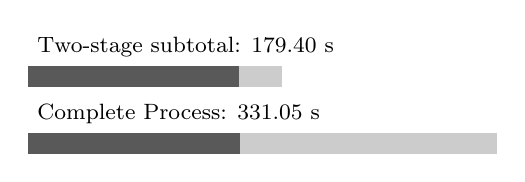
\begin{tikzpicture}[x=0.018cm,y=0.61cm,font=\footnotesize]
\fill[black!65] (0,1) rectangle (148.83,1.43);
\fill[black!20] (148.83,1) rectangle (179.40,1.43);
\node[anchor=west] at (0,1.83) {Two-stage subtotal: 179.40 s};
\fill[black!65] (0,-0.4) rectangle (149.5633,.03);
\fill[black!20] (149.5633,-0.4) rectangle (331.048,.03);
\node[anchor=west] at (0,.44) {Complete Process: 331.05 s};
\end{tikzpicture}
\caption{Historical fixed-input GEMM routing evaluation. Dark bars
show construction. The upper bar adds separate median construction
(148.83 s) and routing (30.57 s) times from different repeats.
The lower bar uses mean construction (149.56 s) and mean Process across the
same three repeats. Loading, initialization, checking, STA and output
enter only the full denominator.}
\label{fig:denominators}\end{figure}
The reservation ended during qualification. All 36 full-process and 18 construction-control timings remain missing. Figure~\ref{fig:denominators} explains why the historical construction shares of 83.0\% and 45.2\% answer different questions. To quantify the opportunity for reducing Process, let $P_r$ and $E_r$ denote Process and E2 of a reference run. Holding other stages fixed, replacing construction with $E'_r$ gives the prediction $P_r/(P_r-E_r+E'_r)$. Setting $E'_r=0$ gives the corresponding upper bound. Comparing predictions to paired Process measurements tests the fixed-remainder assumption.
\subsection{Backend Comparison: ALT CPU versus ALT CUDA}
Both backends receive the same ordered jobs and use shift 20. CPU workers own independent scratch state, whereas the GPU batches all samples and uses atomic whole-pair proposals. Their paired E2 ratio charges the GPU for preparation, transfer and synchronization. Their Process ratio also reflects downstream routing and STA. Unified backend measurements are pending.
\subsection{3D RRG Characteristics and Workload Generalization}

The XML represents vertical connectivity through resources with a layer span. All three graphs have zero edges between disjoint endpoint layer intervals. GEMM has more than twice as many nodes as either recurrent LSTM or binarized BNN. This range changes dense scratch and scan costs while keeping layer count fixed. Performance on three-layer devices remains open.
\subsection{Correctness, QoR and Applicability}\label{sec:applicability}
Auxiliary qualified maps contain 50,789, 24,434 and 23,111 changed congestion words between STRICT and ALT for GEMM, BNN and LSTM, respectively. Delay words and missing-state masks agreed in these comparisons. Changing a representative can change a route trajectory, so each route requires its own legality and QoR record. On the reserved worker, BNN Stock and Pipeline yielded identical wire maps. The ALT CPU and CUDA captures agreed across all 40 contexts, and their wire maps agreed. All four BNN routes had zero overuse and passed independent native FULL checking and STA. Each BNN log also reports 1,314 CHANZ nodes with no fan-in during graph loading. Stock and all candidates had CPD 11.0943 ns. Relative to Stock, wirelength changed by $+0.091\%$ for Pipeline and $+0.068\%$ for each ALT backend. GEMM Stock completed qualification routing, but its Pipeline invocation was interrupted. LSTM qualification and formal QoR across the three cases remain open. Valid lookahead caches remove the need for fresh construction. The GPU implementation also requires dense state for all samples to fit device memory.

\section{Conclusion}
Source-relative recording and ordered tie resolution permit cross-group scheduling when each native flood retains private state. Whole-pair FP32 waves expose a distinct opportunity within each flood, with explicit numerical admission and bucket closure. The input audit establishes three two-layer graphs and the BNN profile quantifies the work induced by coarser scheduling. On these two-layer graphs, the same-rule CPU/CUDA comparison yields construction speedups of 3.31 and 3.18. Ordered STRICT consumption provides a conditional native-map guarantee, while ALT requires independent route qualification.
The 36 primary GEMM and BNN runs establish matched performance. LSTM extends the auxiliary map and backend checks.


\bibliographystyle{IEEEtran}
\bibliography{references}
\end{document}
